\documentclass[12pt]{article}
\usepackage{graphicx}
\usepackage{amsmath}

\begin{document}
CSCI-4100 Assignment 10 Yichuan Wang RIN:661414395\\
EXERCISES\\\\
6.1\\%DONE
(a) High cosine similarity and low Euclidean similarity: A long vector and a short vector both pointing at the same direction. \\

	In this case, the cosine similarity will be 1 since two vectors are 0 degrees apart, while the Euclidean similarity is low since the vectors are very different in length, which results in a high Euclidean distance and therefore low Euclidean similarity. \\
	
	Low cosine similarity and high Euclidean similarity: Two short vectors pointing at exact opposite directions.\\
	
	In this case, the cosine similarity will be -1 according to dot product calculation, yet the Euclidean similarity is relatively high since the Euclidean distance between the tips of two short vectors is small. \\\\
	NOTE: In both cases above the vectors are assumed to start from one same origin.\\\\
(b) A shift of the origin would change the cosine similarity since the position of the origin affects the angle between vectors. Euclidean similarity won't be affected since the shift of origin doesn't change the relative position of two vector tips. \\\\ %6.2 DONE
6.2 When $\pi(x)\geq \frac{1}{2}$, we have $f(x)=1$, $e(f(x))=1-\pi(x)$ and $\pi(x)\geq 1-\pi(x)$; we thus can conclude $e(f(x))=min(\pi(x),1-\pi(x))$.\\
 	When $\pi(x)< \frac{1}{2}$, we have $f(x)=-1$, $e(f(x))=\pi(x)$ and $\pi(x)< 1-\pi(x)$; we thus can conclude $e(f(x))=min(\pi(x),1-\pi(x))$.\\
 	We can now conclude that $e(f(x))=min(\pi(x),1-\pi(x))$ holds for all possible $\pi(x)$.\\
 	$e(f(x))$ is by definition the smallest error since it contains only stochastic noise which cannot be learned at all; therefore any other hypothesis that differs with $f(x)$ is only creating more errors instead of reducing them.\\\\\\ 
PROBLEMS\\
6.1 NOTE: Description is for the picture above it\\%DONE
(a)\\
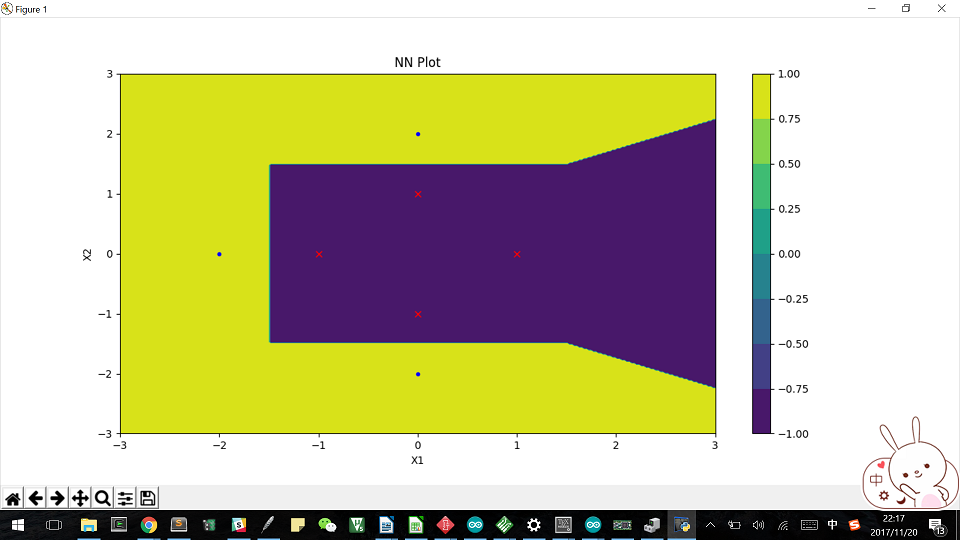
\includegraphics[scale=0.9]{images/1nn_no_tran}\\
1-NN without transform\\\\
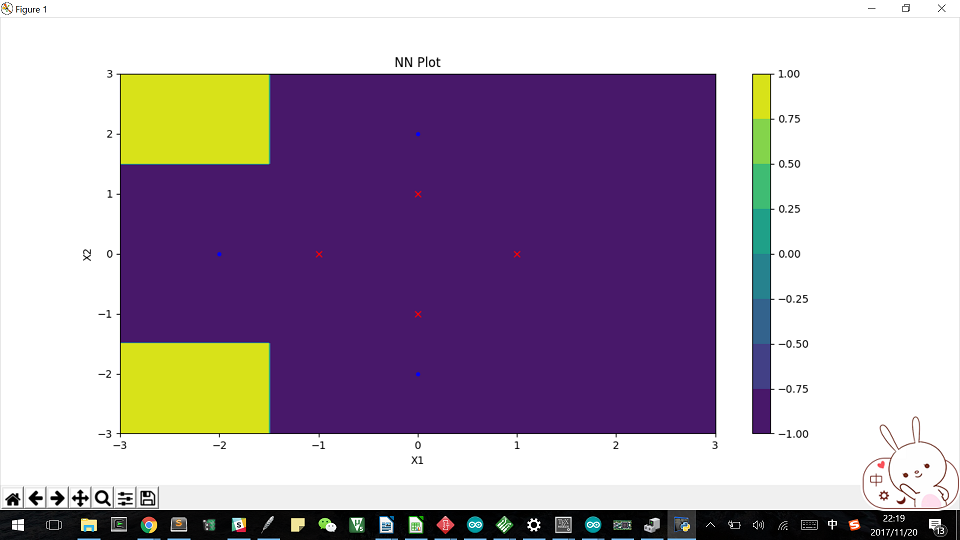
\includegraphics[scale=0.9]{images/3nn_no_tran}\\
3-NN without transform\\
(b)\\
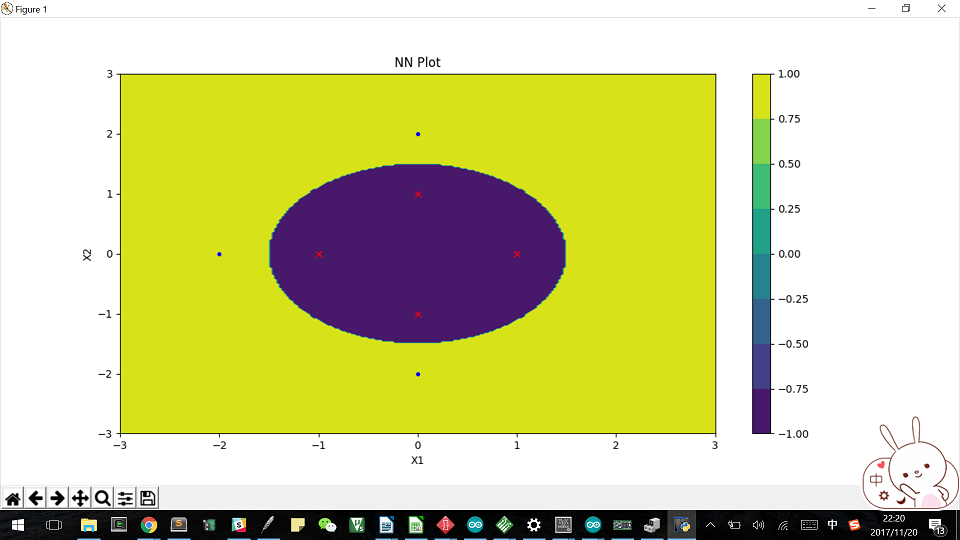
\includegraphics[scale=0.9]{images/1nn_yes_tran}\\
1-NN with transform\\\\
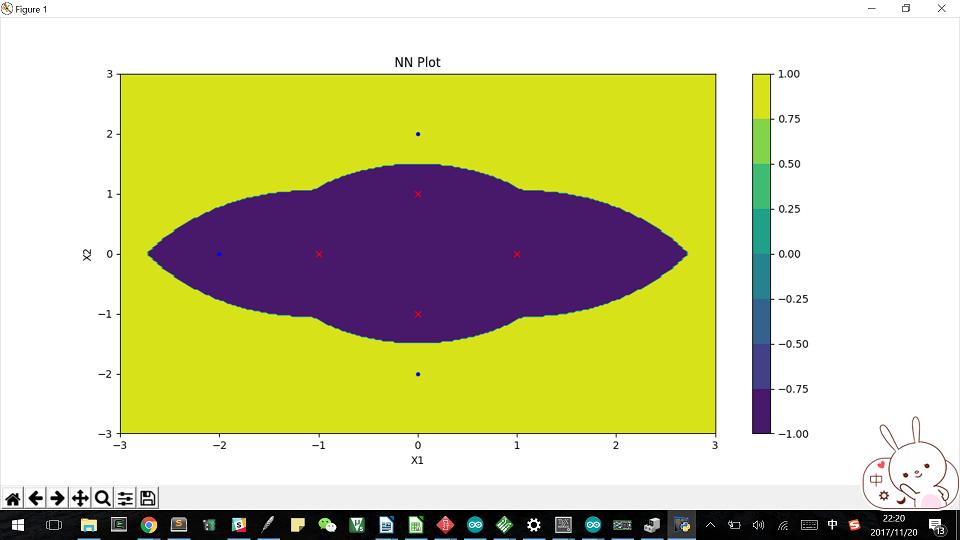
\includegraphics[scale=0.9]{images/3nn_yes_tran}\\
3-NN with transform\\\\\\\\\\\\\\\\\\\\\\\\\\\\\\\\\\\\\\\\
6.4 NOTE: Description is for the picture above it\\%DONE
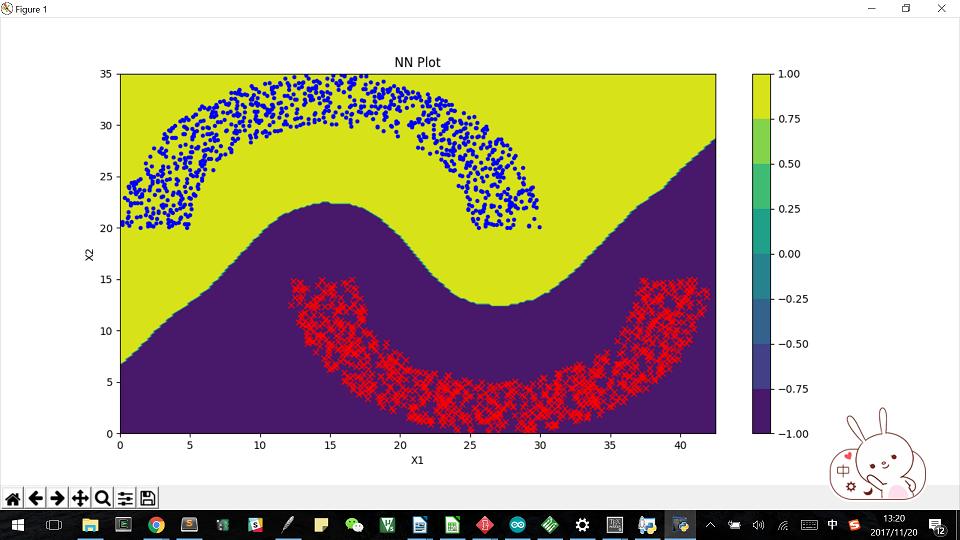
\includegraphics[scale=0.9]{images/6_4_1nn}\\
1-NN case. \\\\
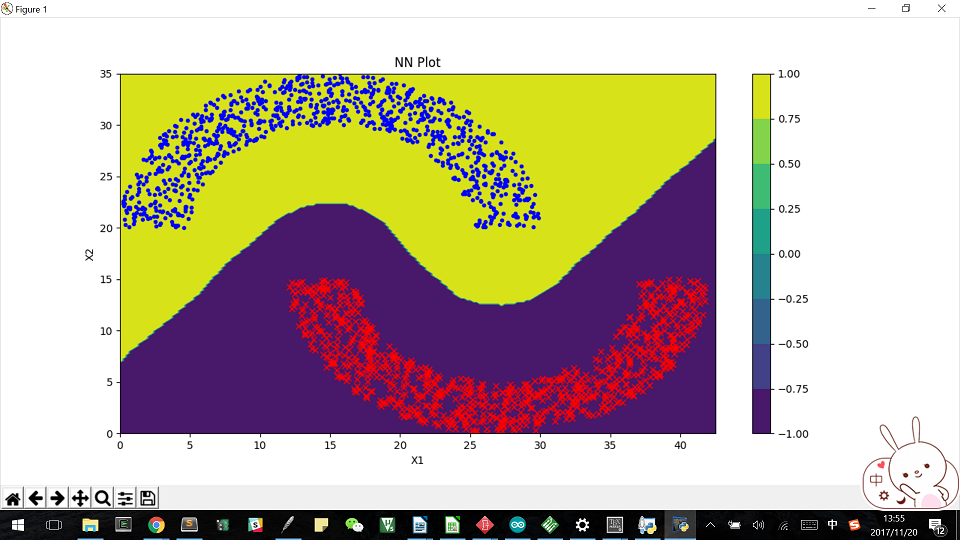
\includegraphics[scale=0.9]{images/6_4_3nn}\\
3-NN case. \\\\
6.16\\%DONE
(a) Both algorithms (10-partition branch and bound versus brute force search) were run on 10000 randomly generated test points. The brute force search takes 538.45 seconds, while the branch and bound search takes 87.96 seconds. The branch bound is clearly faster than brute force search due to its ability to judge and skip large portions of data points.\\\\
(b) Part(a) is repeated with random gaussians clusters with fixed and identical variances. The brute force search takes 563.28 seconds, while the branch and bound search takes 75.83 seconds. The performance of brute force search remains relatively unchanged, while the branch and bound algorithm is around 16 percent faster. This improvement of performance is probably due to better clustering of gaussian cluster data compare to completely random data used in part(a). \\\\
(c) The observations are explained in part(a) and (b)\\\\
(d) No, the number of test point doesn't affect the choice of algorithm. The branch and bound will usually perform better than brute force search since the former can avoid scanning a large portion of unnecessary points. If the data is well clustered, the branch and bound will perform even better.

\end{document}












